\documentclass[12pt,addpoints]{guia}
\grado{2$^\circ$ de Secundaria}
\cicloescolar{2022-2023}
\materia{Ciencias y Tecnología: Física}
\guia{8}
\unidad{3}
\title{Las galaxias}
\aprendizajes{\item Describe cómo se lleva a cabo la exploración de los cuerpos celestes por medio de la detección
de las ondas electromagnéticas que emiten.\item Describe algunos avances en las características
y composición del Universo (estrellas, galaxias y otros sistemas).}
\author{JC Melchor Pinto}
\begin{document}
\INFO%
\begin{sectionbox}{Las galaxias}
    \begin{wrapfigure}[14]{r}[1mm]{0.3\textwidth}
        \centering
        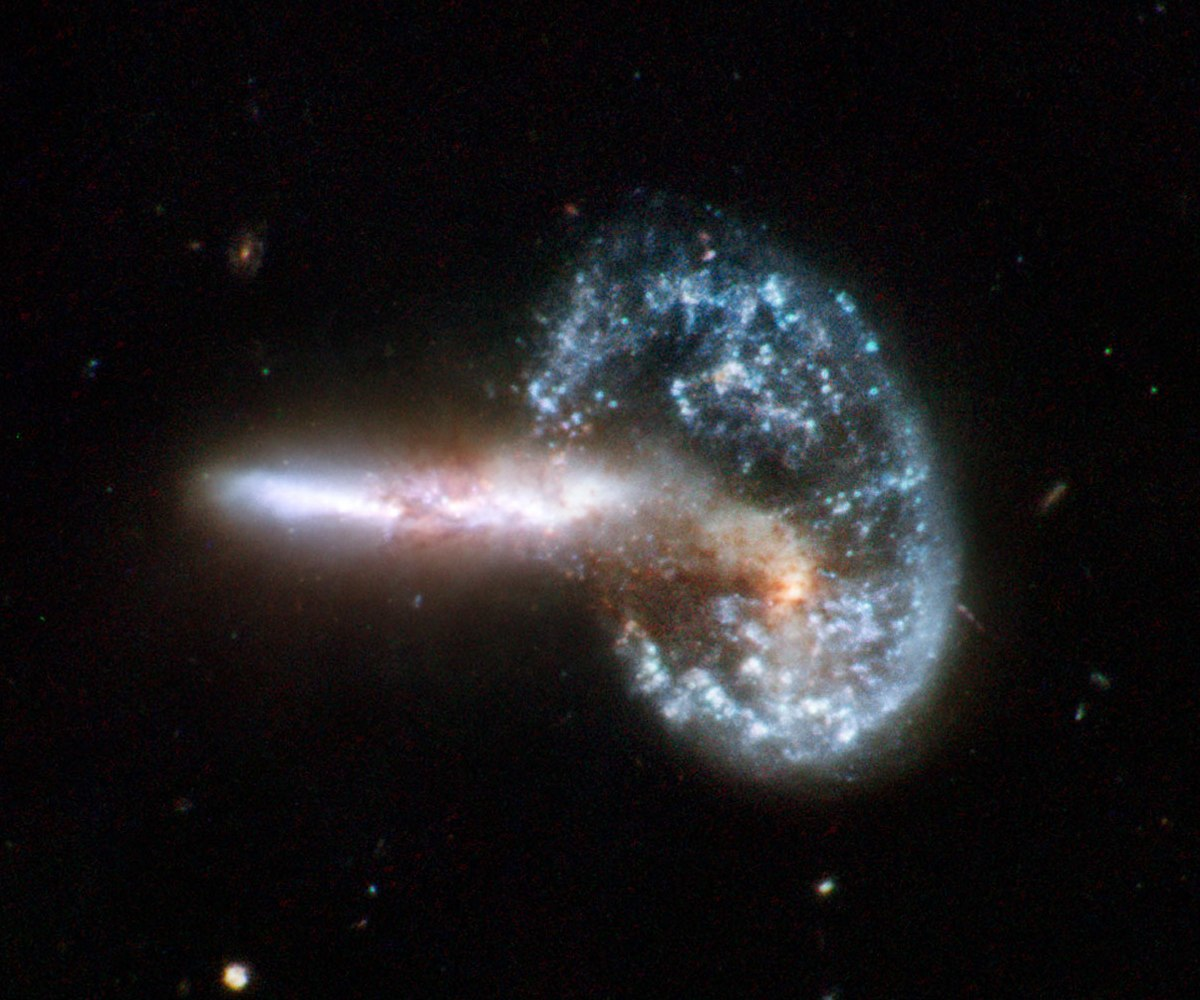
\includegraphics[width=\linewidth]{../images/fusion-galaxie-arp148}
        \caption{Galaxias en colisión.}
        \label{fig:fusion-galaxie-arp148}
    \end{wrapfigure}
    A gran escala, los objetos más grandes del Universo son las galaxias.
    \label{085a_a}Una galaxia es un sistema de estrellas, gas y polvo
    interestelar que orbita en torno a un centro de gravedad.
    Se estima que cada galaxia contiene entre miles y cientos de miles de millones de estrellas; es de esperar, por
    tanto, que muestren comportamientos físicos complejos.

    Desde 1990, gracias al telescopio espacial Hubble y otros
    similares, disponemos de imágenes de las galaxias, algunas
    incluso muy lejanas (figura \ref{fig:fusion-galaxie-arp148}). A partir de esas imágenes se ha inferido que pueden colisionar y fusionarse o atravesarse mutuamente en escalas de tiempo enormes en comparación
    con una vida humana; también sus escalas de
    longitud son colosales, por lo cual conviene usar una unidad de medida adecuada, como el año luz.
    \label{085a_b}El \textbf{año luz} es la unidad de \label{085a_c} longitud que se define como la distancia que la luz recorre en un año. Además de ser útil para
    referir grandes distancias en el Universo, esta unidad indica
    cuánto tiempo tarda la luz y otras ondas electromagnéticas
    en recorrer la distancia referida.
    \begin{wrapfigure}[16]{l}[1mm]{0.55\textwidth}
        \centering
        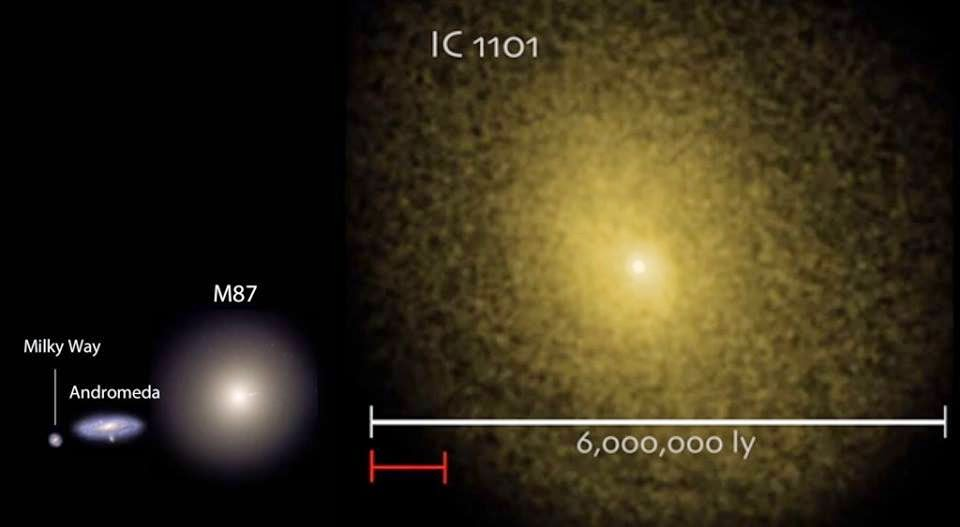
\includegraphics[width=\linewidth]{../images/10301186_1559077347670728_4400880990486792799_n.jpg}
        \caption{Comparación del tamaño de la galaxia más
            grande conocida con los de la Vía Láctea (Milky Way), Andrómeda y Virgo A (M87).}
        \label{fig:10301186_1559077347670728_4400880990486792799_n}
    \end{wrapfigure}

    El tamaño de las galaxias y su número de estrellas varian, lo mismo que otras de sus caracteristicas como la forma.
    La galaxia más grande descubierta hasta hoy (2018) es 1C 1101 (figura \ref{fig:10301186_1559077347670728_4400880990486792799_n}), una galaxia elíptica supergigante, 60 veces más grande que la nuestra; alberga cientos de millones de estrellas. Ubicada en el cúmulo Abell 2029, a mil millones de años luz de la Tierra, fue descubierta en 1790 por William Herschel.
    En cambio se estima que \emph{Segue 2}, la galaxia más pequeña conocida hasta el momento, contiene apenas unas mil estrellas, y se encuentra en la constelacion de Aries, a unos 110 mil años luz de la Tierra; fue descubierta en 2009 usando datos del SPSS.

    En la actualidad se estima que el número de galaxias en el Universo observable es de más de un \label{085a_d}billón separadas entre sí por distancias enormes, del
    orden de millones de años luz, y el espacio entre ellas tiene una densidad
    de materia muy baja, menor que un núcleo de hidrógeno por metro cúbico.
    ¿Cuántas galaxias existirán en el Universo?

    Las galaxias presentan una estructura interna conformada principalmente por un núcleo,
    alrededor del cual orbitan estrellas, polvo y
    gas, como se muestra en la figura \ref{fig:20230521214652}. \label{085a_e} Todo esto constituye apenas 10\% de la
    masa total de la galaxia; \label{085a_f} el 90\% restante esta
    distribuida en un halo que la cubre y no es detectable por su emisión de luz u otras ondas
    electromagnéticas, por lo cual esta masa misteriosa se denomina \textbf{materia oscura}; sin embargo, si ha sido posible saber de su existencia
    por la manera en que afecta la rotación de las
    estrellas más alejadas del núcleo galáctico.

    \begin{figure}[H]
        \centering
        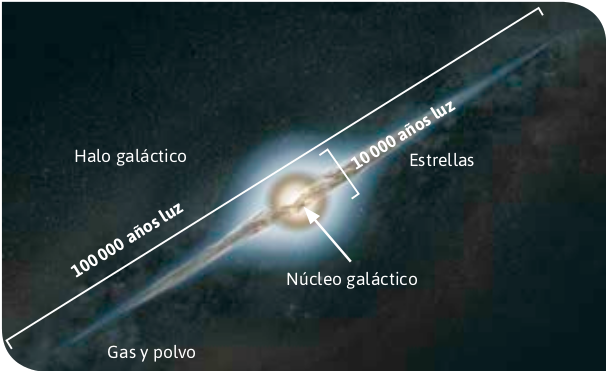
\includegraphics[width=0.65\linewidth]{../images/20230521214652}
        \caption{Estructura de una galaxia, como la Vía Láctea.}
        \label{fig:20230521214652}
    \end{figure}

    % \begin{figure}[H]
    %     \centering
    %     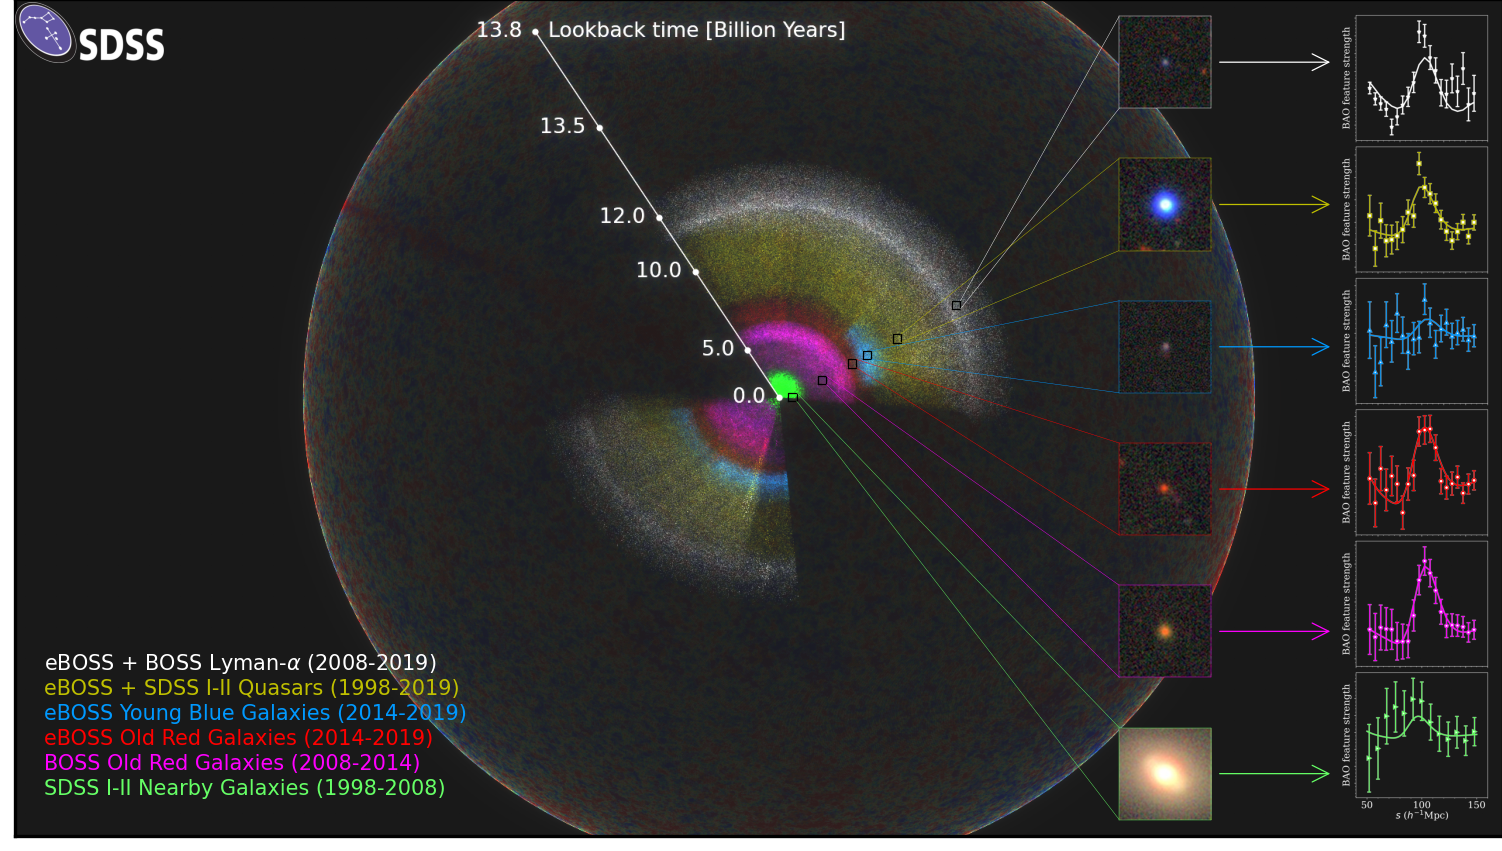
\includegraphics[width=\linewidth]{../images/eboss_pr_v14}
    %     \caption{El mapa del SDSS se muestra como un arco iris de colores, ubicado dentro del Universo observable (la esfera exterior, que muestra las fluctuaciones en el fondo cósmico de microondas). Estamos situados en el centro de este mapa. El recuadro para cada sección del mapa codificada por colores incluye la imagen de una galaxia o cuásar típico de esa sección, y también la señal del patrón que el equipo de eBOSS mide allí. Al mirar a lo lejos, miramos hacia atrás en el tiempo. Por lo tanto, la ubicación de estas señales revela la tasa de expansión del Universo en diferentes momentos de la historia cósmica. Créditos: Anand Raichoor (EPFL), Ashley Ross (Ohio State University) y SDSS.}
    %     \label{fig:eboss_pr_v14}
    % \end{figure}
\end{sectionbox}
\begin{questions}
    \questionboxed[30]{\include*{../questions/question085c}}
    \questionboxed[60]{\include*{../questions/question085a}}
    % \begin{sectionbox}{Tipos de galaxias}
    %     A partir de la observacion de las galaxias se han estable- cido algunos tipos con base en su forma. Una clasificacion muy usada es la que ideo Edwin Hubble (1889-1953) a principios del siglo xx, la cual las divide en tres tipos ba- sicos: elipticas, espirales y espirales barradas (figura 3.50). En los tipos elipticos el numero indica la forma aparente de la galaxia vista desde la Tierra: EO corres- ponde a una forma esférica, y el numero crece hasta E7, lo que indica una forma eliptica cada vez mas alargada. En el caso de las espirales y espirales barradas, la distin- cidn se basa en la separacion de los brazos de las galaxias.
    %     El sistema de clasificacién de Hubble incluia también las galaxias lenticulares, cuya forma es de disco.
    %     También hay otras maneras, para describir a las galaxias que no se basan en la forma. En las que se forma una gran cantidad de estrellas excepcionalmente alta se denomi- nan galaxias con brote estelar. Con un criterio distinto, aquellas galaxias cuyos nucleos muestran una notable emision de radiacion electromagnética se conocen como galaxias activas (figura 3.51).
    %     Las galaxias elipticas se caracterizan, entre otras razones, por tener poco material interestelar y baja formacion de estrellas, en comparacion con las espirales.
    % \end{sectionbox}
    \questionboxed[10]{\include*{../questions/question085b}}
\end{questions}
\end{document}